% ============================================================
%  Chapter 1 -- Introduction to Bayesian Machine Learning
%              in Quantitative Finance
%  Bayesian Machine Learning in Quantitative Finance:
%  Theory and Practical Applications (Springer, 2025)
%  Mongwe, Mbuvha & Marwala
%  Beamer slides -- pdflatex compatible
% ============================================================
\documentclass[aspectratio=169,10pt]{beamer}

\usetheme{Madrid}
\usecolortheme{seahorse}
\usefonttheme{professionalfonts}
\setbeamertemplate{footline}[frame number]
\setbeamertemplate{navigation symbols}{}

% ── packages ────────────────────────────────────────────────
\usepackage{amsmath,amssymb,amsfonts}
\usepackage{bm}
\usepackage{graphicx}
\usepackage{booktabs}
\usepackage{listings}
\usepackage{xcolor}
\usepackage{tikz}
\usetikzlibrary{arrows.meta,positioning,shapes.geometric,calc}
\usepackage{array}
\usepackage{hyperref}

\graphicspath{{figures/}}

% ── listings style ──────────────────────────────────────────
\lstset{
  language=Python,
  basicstyle=\ttfamily\scriptsize,
  numbers=left,
  numberstyle=\tiny\color{gray},
  frame=single,
  backgroundcolor=\color{gray!7},
  keywordstyle=\color{blue!80!black}\bfseries,
  commentstyle=\color{green!50!black}\itshape,
  stringstyle=\color{orange!80!black},
  showstringspaces=false,
  tabsize=2,
  breaklines=true,
  breakatwhitespace=true,
  numbersep=6pt,
}

% ── convenience macros ──────────────────────────────────────
\newcommand{\Real}{\mathbb{R}}
\newcommand{\Prob}{\mathbb{P}}
\newcommand{\Ex}{\mathbb{E}}
\newcommand{\thetav}{\theta}
\newcommand{\Data}{\mathcal{D}}

% ── title ───────────────────────────────────────────────────
\title[Bayesian ML in QF -- Ch.1]{Bayesian Machine Learning in Quantitative Finance}
\subtitle{Chapter 1: Introduction}
\author{Based on Mongwe, Mbuvha \& Marwala}
\date{}

% ============================================================
\begin{document}
% ============================================================

\begin{frame}
  \titlepage
\end{frame}

\begin{frame}{Outline}
  \tableofcontents
\end{frame}

% ============================================================
\section{Notation and Background}
% ============================================================

\begin{frame}[allowframebreaks]{Notation and Background You Need}
  This chapter assumes only basic probability. Everything else is built up
  from scratch here. Keep this frame as a reference for the rest of the book.

  \begin{block}{Frequentist vs.\ Bayesian thinking (the big picture)}
    \begin{itemize}
      \item \textbf{Frequentist view:} an unknown quantity (e.g.\ a model
      parameter) has one true, fixed value. We estimate it from data and
      report how our estimate would vary if we repeated the experiment.
      \item \textbf{Bayesian view:} an unknown quantity is treated as
      \emph{uncertain}, and we describe our uncertainty about it using a
      probability distribution. \textbf{Bayesian inference} is simply the
      process of \emph{updating a belief about an unknown, using data} --
      we start with a belief, observe evidence, and end with a revised
      belief.
    \end{itemize}
  \end{block}

  \framebreak

  \begin{block}{The four ingredients of Bayes' theorem (plain English)}
    \begin{itemize}
      \item \textbf{Prior} $\Prob(\thetav)$ -- what you believed about the
      unknown $\thetav$ \emph{before} seeing any data. One-line analogy:
      your ``gut feeling'' or existing evidence walking into the experiment.
      \item \textbf{Likelihood} $\Prob(\Data \mid \thetav)$ -- how probable
      the observed data $\Data$ would be, \emph{for each candidate value} of
      $\thetav$. One-line analogy: ``if $\thetav$ were true, how surprising
      would this data be?''
      \item \textbf{Posterior} $\Prob(\thetav \mid \Data)$ -- your
      \emph{updated} belief about $\thetav$ \emph{after} seeing the data.
      One-line analogy: prior belief, corrected in light of evidence.
      \item \textbf{Evidence} $\Prob(\Data)$ -- the overall probability of
      the data, averaged over all possible values of $\thetav$. It is just a
      normalizing constant, but it turns out to be very useful for
      \emph{comparing models}.
    \end{itemize}
  \end{block}

  \framebreak

  \begin{block}{Bayes' theorem, written out and labeled}
    \[
      \underbrace{\Prob(\thetav \mid \Data)}_{\text{posterior}}
      \;=\;
      \frac{\overbrace{\Prob(\Data \mid \thetav)}^{\text{likelihood}}
      \;\times\;
      \overbrace{\Prob(\thetav)}^{\text{prior}}}
      {\underbrace{\Prob(\Data)}_{\text{evidence}}}
    \]
    where $\Prob(\Data) = \int \Prob(\Data \mid \thetav)\, \Prob(\thetav)\, d\thetav$
    sums (integrates) the numerator over every possible $\thetav$, so that
    the posterior is a valid probability distribution (it integrates to 1).
  \end{block}

  \textbf{Why this matters for this book:} every Bayesian machine learning
  method in the chapters ahead -- Markov Chain Monte Carlo (MCMC),
  variational inference, Gaussian processes, normalizing flows, Bayesian
  neural networks -- is, at its core, just a clever way of computing or
  approximating this posterior when the exact formula above is too hard to
  evaluate directly.
\end{frame}

% ============================================================
\section{1.1 Introduction}
% ============================================================

\begin{frame}[allowframebreaks]{Why Machine Learning Meets Quantitative Finance}
  \begin{block}{Intuition}
    We are in the middle of a technology wave (the ``fourth industrial
    revolution'') where artificial intelligence and cyber-physical systems
    are reshaping entire industries. Machine learning -- algorithms that
    learn input-output mappings directly from data, most prominently neural
    networks -- is the engine behind this wave, and finance is no exception.
  \end{block}

  \begin{block}{What is quantitative finance?}
    A cross-disciplinary field that borrows tools from computer science,
    physics, statistics, and mathematics to solve real-world finance
    problems. Traditionally, quantitative models are \emph{parsimonious} and
    \emph{interpretable} -- they are grounded in economic theory so
    practitioners can explain why a model behaves the way it does.
  \end{block}

  \begin{block}{The sell-side / buy-side split}
    Quantitative finance applications broadly split into:
    \begin{itemize}
      \item \textbf{Sell-side} -- where financial product structures (e.g.\
      derivatives) are \emph{constructed}.
      \item \textbf{Buy-side} -- where those constructed products are
      \emph{consumed} (e.g.\ by investors and asset managers).
    \end{itemize}
    This book explores methods relevant to both.
  \end{block}
\end{frame}

\begin{frame}[allowframebreaks]{A Short History: From Bachelier to Deep Hedging}
  Derivative pricing is one of the oldest and richest applications of
  quantitative methods in finance -- a useful case study of how the field
  has evolved, and where Bayesian thinking now fits in.

  \begin{itemize}
    \item \textbf{Bachelier (1900):} the founding work of mathematical
    finance. Modeled asset price changes using Brownian motion, predating
    Einstein's own work on the topic. Drawback: it allowed asset prices to
    go negative -- a flaw that seemed fatal for decades, until
    negative-interest-rate environments made it relevant again.
    \item \textbf{Black \& Scholes (1973):} the breakthrough model, and
    still the standard reference for pricing and risk-managing options. Key
    (strong) assumption: volatility is \emph{constant} over the life of the
    option -- no skew, no term structure.
    \item \textbf{Market crises exposed the flaw:} major market crises led
    to a persistent \emph{volatility skew}, invalidating the constant-volatility
    assumption. This triggered an explosion of richer models built to
    capture the skew, such as the Heston stochastic volatility model and
    jump-diffusion processes.
  \end{itemize}

  \framebreak

  \begin{itemize}
    \item \textbf{Data-driven era:} more recently, machine learning has
    entered derivative pricing and risk management directly. A landmark
    result is \emph{deep hedging} (Buehler et al., 2019), which showed deep
    learning could be used to hedge options successfully. Other work uses
    machine learning to price exotic instruments, calibrate rough
    stochastic volatility models, and generate synthetic market data with
    generative adversarial networks.
    \item \textbf{The gap this book targets:} most of these data-driven
    approaches produce \emph{point estimates} -- a single number, with
    little to no exploration of \emph{uncertainty}. Bayesian methods
    naturally encapsulate uncertainty in both parameter estimates and model
    outputs, which is exactly what is missing.
  \end{itemize}
\end{frame}

\begin{frame}[allowframebreaks]{Beyond Derivatives: Where Else Finance Meets ML}
  The book's motivation is not limited to derivatives -- similar
  data-driven trends and the same need for principled uncertainty appear
  across quantitative finance.

  \begin{block}{Asset management / portfolio theory}
    Modern portfolio theory (Markowitz), the Capital Asset Pricing Model
    (Sharpe, Lintner), and Fama--French factor models are the classical
    foundations. Machine learning has recently been used to build
    ML-augmented CAPM models, combine sell-side analyst forecasts more
    accurately, and improve short-horizon stock-price direction forecasts
    using limit order book data.
  \end{block}

  \begin{block}{Credit risk}
    Banks have traditionally used logistic regression for loan default
    modeling -- driven largely by regulatory requirements that credit
    decisions be explainable to customers. Tree-based methods (random
    forests, boosted trees) are being explored, but full neural networks
    have seen low uptake because of their ``black-box'' nature. Recovery on
    defaulted loans has traditionally used Beta regression and zero-inflated
    models; corporate credit ratings (from agencies like Moody's and S\&P)
    are also being modeled with trees and neural networks as
    cost-effective alternatives to expert-driven rating processes.
  \end{block}

  \framebreak

  \begin{block}{Financial management}
    Sound financial management is essential to organizational
    sustainability. High-profile scandals (Enron, Wirecard, Steinhoff, and
    others) and repeated audit failures in public institutions show the
    cost of poor oversight. Machine learning methods -- logistic
    regression, support vector machines, Na\"ive Bayes, neural networks --
    have been used to model audit opinions; modeling \emph{unlawful
    expenditure} specifically is still a comparatively open research area.
  \end{block}

  \begin{block}{Insurance}
    Insurance is fundamentally a risk-transfer mechanism: a policyholder
    pays a fee to transfer an insurable risk to the insurer. Machine
    learning has been applied to address data limitations (e.g.\ class
    imbalance via generative adversarial networks), model mortality,
    improve motor claim predictions, and reduce risk in weather-index
    insurance products.
  \end{block}
\end{frame}

\begin{frame}[allowframebreaks]{The Open Questions Motivating This Book}
  \begin{block}{Intuition}
    As machine learning models proliferate across quantitative finance, a
    common set of hard questions keeps resurfacing -- questions that
    standard (point-estimate) machine learning struggles to answer well.
  \end{block}
  \begin{block}{The four questions}
    \begin{enumerate}
      \item How can we \textbf{explain} the prediction or output of a model?
      \item What is the \textbf{distribution} of the model's parameters
      (not just a single best-fit value)?
      \item How do we \textbf{select between competing models} in a
      statistically principled way?
      \item Which \textbf{inputs} are most relevant to the task at hand?
    \end{enumerate}
  \end{block}
  \begin{block}{This book's answer}
    The \textbf{Bayesian inference framework}. As we will see, the four
    components of Bayes' theorem map naturally onto these four questions --
    the posterior gives us parameter and prediction distributions, the
    likelihood encapsulates the model and adapts to new data, the prior can
    automatically highlight relevant inputs, and the evidence lets us
    compare models on principled grounds.
  \end{block}
\end{frame}

% ============================================================
\section{The Toy Example: A Coin Flip}
% ============================================================

\begin{frame}{Running Example: Is This Coin Fair?}
  \begin{block}{Intuition}
    Before diving into finance, let's build intuition with the simplest
    possible Bayesian problem. It has exactly the same structure as
    everything else in this book -- just with much smaller math.
  \end{block}
  \begin{block}{The setup}
    \begin{itemize}
      \item Unknown parameter: $\thetav \in [0,1]$, the probability the
      coin lands heads.
      \item \textbf{Prior belief:} we think the coin is probably close to
      fair, but we are not certain -- we encode this as a prior distribution
      centered at $\thetav = 0.5$ (not a single fixed guess).
      \item \textbf{Data:} we flip the coin 10 times and observe
      \textbf{8 heads and 2 tails}.
      \item \textbf{Question:} how should our belief about $\thetav$ change?
    \end{itemize}
  \end{block}
  \textbf{Preview:} we will see much more sophisticated versions of this
  exact same idea throughout the book -- the ``coin'' will become an
  option's implied volatility parameter, a credit rating, an audit outcome,
  or a claims-frequency rate, and the simple formula on the next slides will
  become variational inference, MCMC, Gaussian processes, normalizing flows
  and Bayesian neural networks.
\end{frame}

\begin{frame}{Bayes' Theorem: The Mechanics (Fig.\ 1.1 style)}
  \begin{block}{Intuition}
    Bayes' theorem is not just a formula -- it is a \emph{recipe}: combine
    what the model says about the data (likelihood) with what you believed
    beforehand (prior), then normalize.
  \end{block}
  \begin{center}
  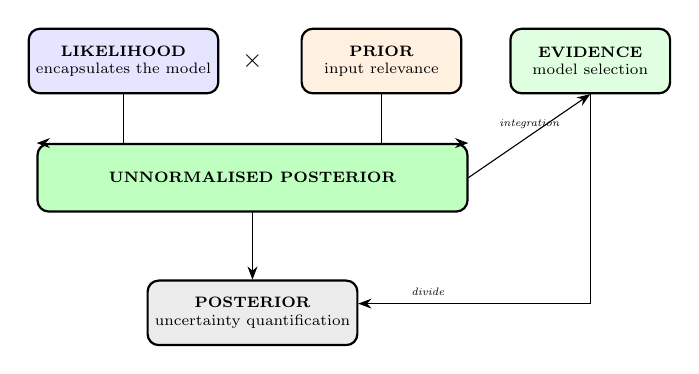
\begin{tikzpicture}[
      scale=0.78, transform shape,
      box/.style={draw, rounded corners, thick, minimum height=1.05cm, minimum width=2.6cm,
                  align=center, font=\scriptsize},
      lbl/.style={font=\tiny\itshape},
      >=Stealth
    ]
    \node[box, fill=blue!10] (like) at (0,3) {\textbf{LIKELIHOOD}\\ encapsulates the model};
    \node[font=\large] (times) at (2.1,3) {$\times$};
    \node[box, fill=orange!12] (prior) at (4.2,3) {\textbf{PRIOR}\\ input relevance};
    \node[box, fill=green!12, minimum width=2.6cm] (evid) at (7.6,3) {\textbf{EVIDENCE}\\ model selection};
    \node[box, fill=green!25, minimum width=7cm, minimum height=1.1cm] (unnorm) at (2.1,1.1) {\textbf{UNNORMALISED POSTERIOR}};
    \node[box, fill=gray!15] (post) at (2.1,-1.1) {\textbf{POSTERIOR}\\ uncertainty quantification};

    \draw[->] (like.south) |- (unnorm.north west);
    \draw[->] (prior.south) |- (unnorm.north east);
    \draw[->] (unnorm.east) -- (evid.south) node[midway,above,lbl]{integration};
    \draw[->] (evid.south) |- ($(post.east)+(0,0.15)$) node[midway,above,lbl,pos=0.85]{divide};
    \draw[->] (unnorm.south) -- (post.north);
  \end{tikzpicture}
  \end{center}
  \small
  The likelihood (model fit to data) is multiplied by the prior (relevance
  of inputs) to give an unnormalised posterior. Integrating that over all
  $\thetav$ gives the evidence (useful for model comparison); dividing by it
  gives the properly normalised posterior (our uncertainty-quantified final
  belief).
\end{frame}

\begin{frame}{Coin Flip: Choosing the Prior and Likelihood}
  \begin{block}{A convenient prior: the Beta distribution}
    We encode ``probably close to fair, but uncertain'' with a
    $\text{Beta}(a_0, b_0)$ prior over $\thetav$:
    \[
      \Prob(\thetav) = \text{Beta}(\thetav \mid a_0, b_0), \qquad
      a_0 = b_0 = 4
    \]
    This distribution is centered at $\tfrac{a_0}{a_0+b_0} = 0.5$ (fair coin)
    but assigns non-trivial probability to other values of $\thetav$ --
    it is a genuine \emph{belief}, not a single guess.
  \end{block}
  \begin{block}{The likelihood of 8 heads out of 10 flips}
    Each flip is a Bernoulli trial, so the data likelihood follows a
    Binomial pattern:
    \[
      \Prob(\Data \mid \thetav) \;\propto\; \thetav^{8} (1-\thetav)^{2}
    \]
    This is \emph{large} for $\thetav$ near $0.8$ (the observed heads rate)
    and \emph{small} for $\thetav$ near 0 or 1 -- exactly what ``how probable
    is this data, for each candidate $\thetav$'' should look like.
  \end{block}
\end{frame}

\begin{frame}{Coin Flip: From Prior to Posterior}
  \begin{block}{Conjugate update (Beta--Binomial)}
    Multiplying a $\text{Beta}(a_0,b_0)$ prior by a Binomial likelihood with
    $h$ heads and $t$ tails gives, after normalizing, another Beta
    distribution:
    \[
      \Prob(\thetav \mid \Data) = \text{Beta}\big(\thetav \mid a_0 + h,\; b_0 + t\big)
    \]
    With $a_0=b_0=4$, $h=8$, $t=2$: posterior $= \text{Beta}(12, 6)$.
  \end{block}
  \centering
  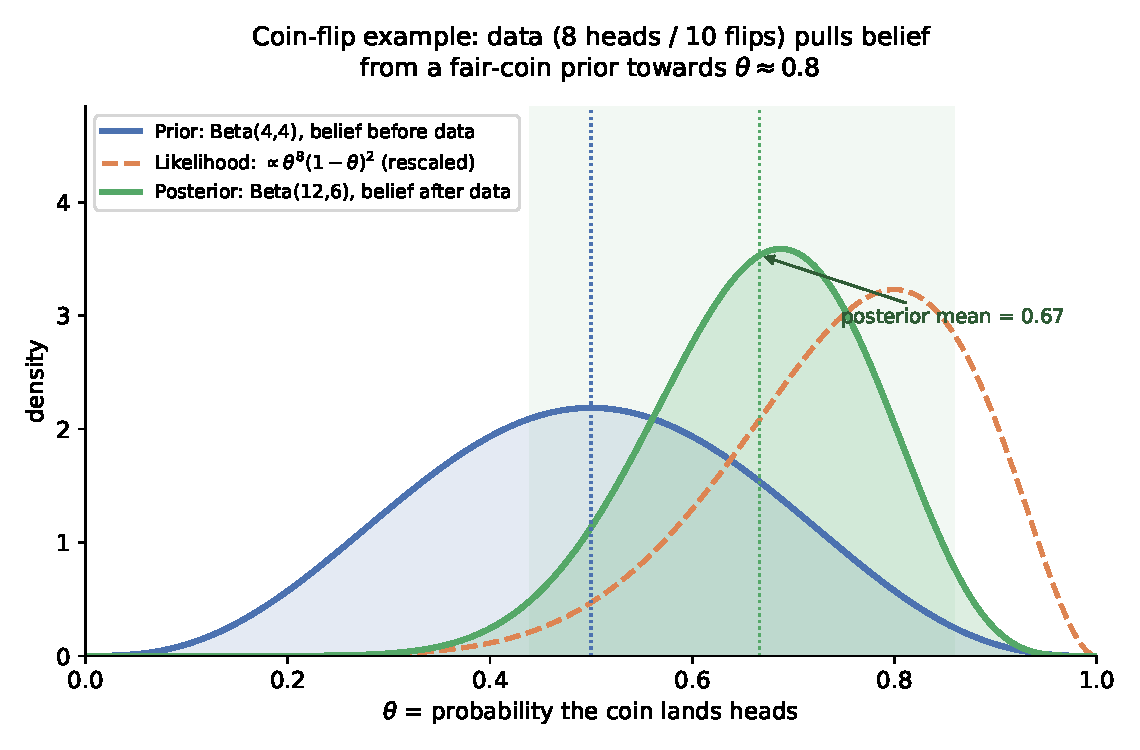
\includegraphics[height=0.48\textheight]{fig_bayes_coin.pdf}
\end{frame}

\begin{frame}{Coin Flip: Reading the Result}
  \begin{block}{Numeric summary}
    \begin{itemize}
      \item Prior mean: $0.500$ (our starting ``fair coin'' belief).
      \item Observed heads rate: $8/10 = 0.800$.
      \item \textbf{Posterior mean: $0.667$} -- pulled from 0.5 towards 0.8,
      but not all the way, because the prior still carries some weight.
      \item 95\% credible interval: approximately $[0.44,\, 0.86]$ -- a
      \emph{range} of plausible values for $\thetav$, not just one number.
    \end{itemize}
  \end{block}
  \begin{block}{Intuition: why not just report $\hat\thetav = 0.8$?}
    A frequentist point estimate would simply report the observed rate,
    $8/10=0.8$, with no sense of how much data (10 flips!) supports that
    number. The Bayesian posterior instead gives a full distribution: it
    shows the estimate \emph{and} how confident we should be in it -- this
    is precisely the kind of uncertainty quantification that later chapters
    exploit for option pricing, credit ratings, audit models, and more.
  \end{block}
\end{frame}

\begin{frame}[fragile]{Python: Coin-Flip Prior-to-Posterior Update}
\begin{lstlisting}
import numpy as np
from scipy.stats import beta

# Prior belief: coin is "probably fair" -> Beta(4,4)
a0, b0 = 4.0, 4.0
# Observed data: 8 heads out of 10 flips
n_flips, n_heads = 10, 8
n_tails = n_flips - n_heads

# Conjugate Beta-Binomial update: posterior is Beta(a0+heads, b0+tails)
a_post, b_post = a0 + n_heads, b0 + n_tails
prior_mean = a0 / (a0 + b0)
post_mean  = a_post / (a_post + b_post)
ci_low, ci_high = beta.ppf([0.025, 0.975], a_post, b_post)

print(f"Prior mean:            {prior_mean:.3f}")        # 0.500
print(f"Observed heads rate:   {n_heads/n_flips:.3f}")    # 0.800
print(f"Posterior mean:        {post_mean:.3f}")          # 0.667
print(f"95% credible interval: [{ci_low:.3f}, {ci_high:.3f}]")  # [0.440, 0.858]

# For plotting: evaluate prior/posterior densities over theta in [0,1]
theta = np.linspace(0.001, 0.999, 500)
prior_pdf = beta.pdf(theta, a0, b0)
post_pdf  = beta.pdf(theta, a_post, b_post)
\end{lstlisting}
\end{frame}

\begin{frame}{From a Coin to Quantitative Finance}
  \begin{block}{The same recipe, over and over}
    Every chapter in this book repeats this exact prior $\to$ likelihood
    $\to$ posterior recipe -- just with $\thetav$ replaced by something
    financially meaningful, and with computational tools replacing the
    simple Beta-Binomial formula when the math is not so friendly:
  \end{block}
  \begin{itemize}
    \item \textbf{MCMC \& variational inference} -- general-purpose ways to
    approximate a posterior when there is no neat closed-form update
    (used throughout the book, starting in Chapter 2).
    \item \textbf{Gaussian processes} -- place a Bayesian ``belief'' over an
    entire unknown \emph{function} (e.g.\ a volatility surface or a credit
    rating function), not just a single parameter.
    \item \textbf{Normalizing flows} -- build flexible, learnable probability
    distributions for prices, model choices, or audit outcomes.
    \item \textbf{Bayesian neural networks} -- neural networks with a
    distribution over their weights, giving uncertainty-aware predictions
    (e.g.\ for insurance claims).
  \end{itemize}
  \small (No technical depth needed yet -- these are previewed here and
  developed fully in later chapters.)
\end{frame}

% ============================================================
\section{1.2 Themes of the Book}
% ============================================================

\begin{frame}{The Book's Four Themes}
  \begin{block}{Intuition}
    The book is organized around four themes, all built on the same
    Bayesian inference framework just introduced, applied to different
    corners of quantitative finance.
  \end{block}
  \centering
  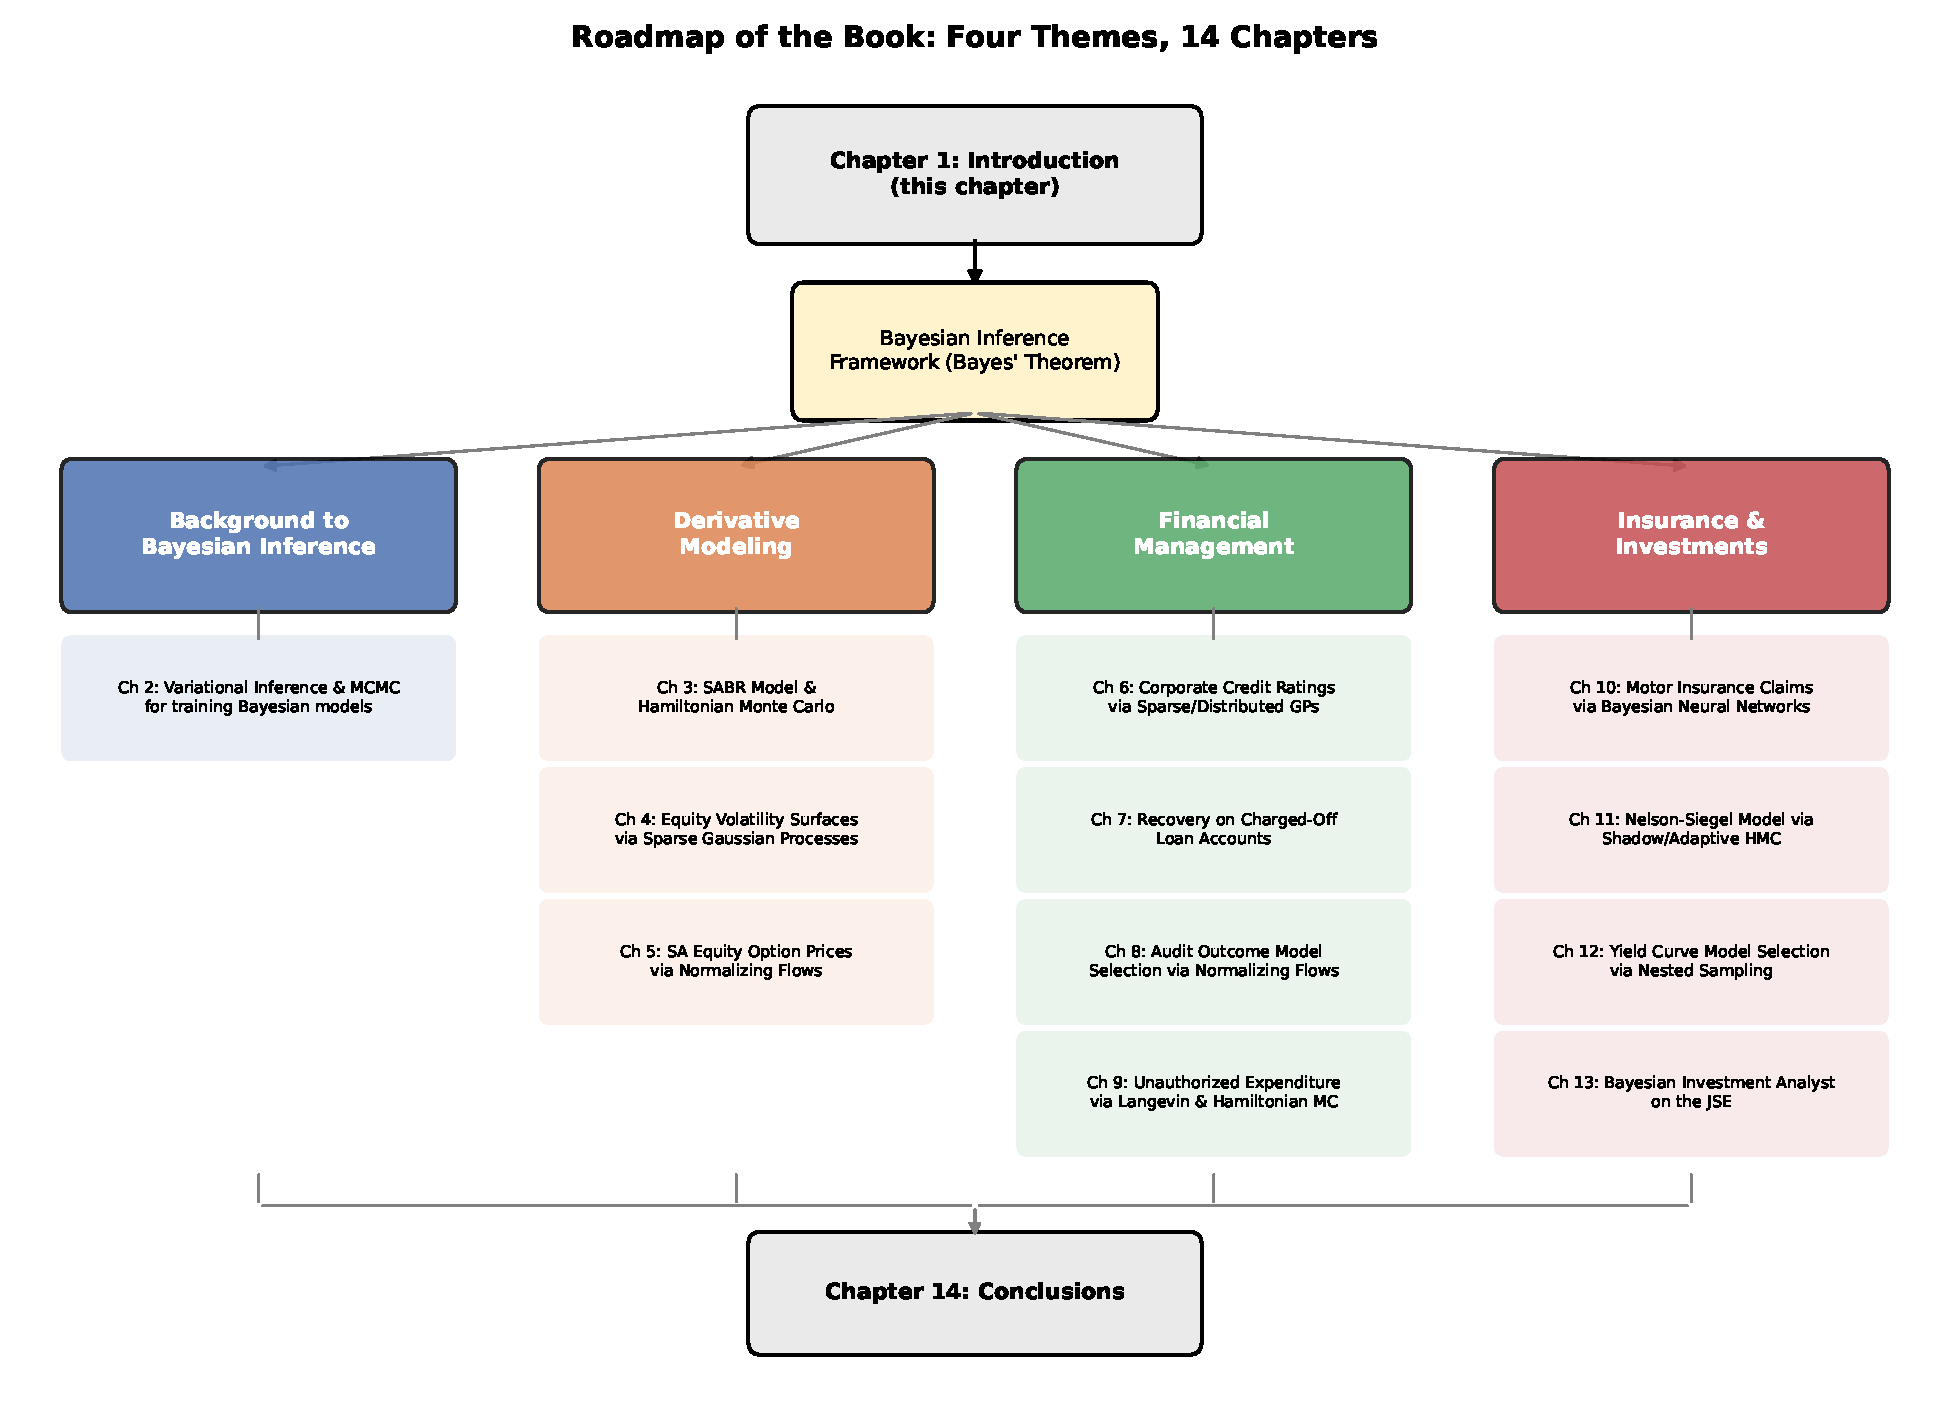
\includegraphics[height=0.65\textheight]{fig_book_roadmap.pdf}
\end{frame}

\begin{frame}{Theme 1: Background to Bayesian Inference}
  \begin{block}{What it covers}
    Before applying Bayesian methods to finance, we need the computational
    machinery to actually \emph{compute} posteriors when there's no simple
    formula (unlike our coin example).
  \end{block}
  \begin{itemize}
    \item \textbf{Chapter 2:} introduces \textbf{variational inference} and
    \textbf{Markov Chain Monte Carlo (MCMC)} techniques used to train
    Bayesian models throughout the rest of the book, together with the
    performance metrics used to assess these inference algorithms.
  \end{itemize}
  \textbf{Why it comes first:} the book is designed so each theme chapter
  can be read in isolation, but all of them depend on the background
  established here -- this is the foundation for everything that follows.
\end{frame}

\begin{frame}{Theme 2: Derivative Modeling}
  \begin{block}{What it covers}
    Applying the Bayesian framework to derivative pricing, model
    calibration, and volatility surface modeling. Benefits highlighted in
    the book: confidence bands on prices, a full distribution over
    calibrated parameters, and no need to bolt on external arbitrage-free
    constraints to the loss function.
  \end{block}
  \begin{itemize}
    \item \textbf{Chapter 3:} the Stochastic Alpha Beta Rho (SABR) model,
    calibrated with Hamiltonian Monte Carlo.
    \item \textbf{Chapter 4:} learning equity volatility surfaces using
    sparse Gaussian processes.
    \item \textbf{Chapter 5:} analyzing South African equity option prices
    using normalizing flows.
  \end{itemize}
\end{frame}

\begin{frame}{Theme 3: Financial Management}
  \begin{block}{What it covers}
    Bayesian tools applied to topics important to banks (credit ratings,
    recoveries on defaulted loans) and to municipal financial management
    (selecting models for audit-outcome prediction and detecting
    unauthorized expenditure).
  \end{block}
  \begin{itemize}
    \item \textbf{Chapter 6:} sparse and distributed Gaussian processes for
    modeling corporate credit ratings.
    \item \textbf{Chapter 7:} Bayesian detection of recovery on charged-off
    loan accounts.
    \item \textbf{Chapter 8:} Bayesian audit outcome model selection using
    normalizing flows.
    \item \textbf{Chapter 9:} Bayesian detection of unauthorized expenditure
    using Langevin and Hamiltonian Monte Carlo.
  \end{itemize}
\end{frame}

\begin{frame}{Theme 4: Insurance and Investments}
  \begin{block}{What it covers}
    Bayesian inference applied to motor insurance claims, calibrating yield
    curve models, and building a Bayesian sell-side investment analyst.
  \end{block}
  \begin{itemize}
    \item \textbf{Chapter 10:} Bayesian neural network inference of motor
    insurance claims.
    \item \textbf{Chapter 11:} shadow and adaptive Hamiltonian Monte Carlo
    methods for calibrating the Nelson-Siegel yield curve model.
    \item \textbf{Chapter 12:} static and dynamic nested sampling for yield
    curve model selection.
    \item \textbf{Chapter 13:} a Bayesian investment analyst on the
    Johannesburg Stock Exchange (JSE).
  \end{itemize}
\end{frame}

% ============================================================
\section{1.3 Conclusion}
% ============================================================

\begin{frame}[allowframebreaks]{Chapter Summary}
  \begin{block}{What this chapter established}
    \begin{itemize}
      \item Machine learning is transforming quantitative finance across
      derivative modeling, portfolio/asset management, credit risk,
      financial management, and insurance.
      \item Most existing data-driven approaches give point estimates only,
      leaving four open questions: explainability, parameter uncertainty,
      principled model selection, and input relevance.
      \item The \textbf{Bayesian inference framework} (prior $\times$
      likelihood, normalized by the evidence) directly addresses all four,
      as shown with our coin-flip toy example (prior mean $0.5 \to$
      posterior mean $0.667$ after 8/10 heads).
      \item The book is organized into four themes: background to Bayesian
      inference, derivative modeling, financial management, and insurance
      and investments, spanning Chapters 2 through 13, with Chapter 14
      drawing overall conclusions.
    \end{itemize}
  \end{block}
  \begin{block}{Looking ahead}
    Chapter 2 provides the computational core the rest of the book leans
    on: variational inference and Markov Chain Monte Carlo methods for
    training Bayesian models, plus the metrics used to judge how well these
    inference algorithms are working.
  \end{block}
\end{frame}

\begin{frame}{Key Takeaways}
  \begin{itemize}
    \item Bayesian inference = updating a belief about an unknown using
    data, via \emph{posterior} $\propto$ \emph{likelihood} $\times$
    \emph{prior}, normalized by the \emph{evidence}.
    \item Even a two-parameter coin-flip example shows the core value:
    a full distribution over the unknown, not just one number.
    \item Quantitative finance is rich with unknowns worth treating this
    way: volatility parameters, credit ratings, recovery amounts, audit
    outcomes, claims rates, yield curve parameters, and more.
    \item This book's four themes progressively build the computational
    tools (MCMC, variational inference, Gaussian processes, normalizing
    flows, Bayesian neural networks) needed to bring Bayesian thinking to
    each of these problems.
  \end{itemize}
\end{frame}

\end{document}
